% ______________________________________________________________________________
%
% DVG001 -- Introduktion till Linux och små nätverk
%                              Inlämningsuppgift #4
% ~~~~~~~~~~~~~~~~~~~~~~~~~~~~~~~~~~~~~~~~~~~~~~~~~
% Author:   Jonas Sjöberg
%           tel12jsg@student.hig.se
%
% Date:     2016-04-06 -- 2016-04-11
%
% License:  Creative Commons Attribution 4.0 International (CC BY 4.0)
%           <http://creativecommons.org/licenses/by/4.0/legalcode>
%           See LICENSE.md for additional licensing information.
% ______________________________________________________________________________


\section{Del ett}
% TODO: introduktion till del 1


% ______________________________________________________________________________
\subsection{\texttt{IP}-nummer}
\subsubsection{Uppgiftsbeskrivning}
Här är uppgiften att ta reda på vilken \texttt{IP}-adress som maskinen har samt
hur den fått sin adress genom att använda kommandot \texttt{ip} och titta i
loggar, exempelvis \texttt{/var/log/messages}.


\subsubsection{Lösning}
För att ta reda på datorns \texttt{IP}-adress körs kommandot i
Programlistning~\ref{listing:sh_1-ip}.

\begin{listing}[H]
  \shellcode{include/sh_1-ip}
  \caption{Kommando för att ta reda på datorns \texttt{IP}-adress.}
  \label{listing:sh_1-ip}
\end{listing}

Resultatet visar att datorns \texttt{IP}-adress är \texttt{192.168.1.112} 
med nätmasken \texttt{24}.

Ett shell-skript används för att söka igenom loggar efter den aktuella
\texttt{IP}-adressen. Programmet letar efter filer i sökvägen \texttt{/var/log}
och undersöker filernas innehåll genom att läsa ''magic header bytes'' som
avgör vilken typ av fil det är. Om en hittad fil är en vanlig textfil söks dess
innehåll efter datorns aktuella \texttt{IP}-adress som extarherats tidigare.

Programmet visas i Programlistning~\ref{listing:sh_1-grep-logs.sh} och
resultatet av en körning visas i
Figur~\ref{fig:sh_1-grep-logs.sh_output}

\begin{listing}[H]
  \shellcode{include/sh_1-grep-logs.sh}
  \caption{Kommando för att söka igenom loggar i sökvägen \texttt{/var/log}
           efter omnämnanden av datorns aktuella \texttt{IP}-adress.}
  \label{listing:sh_1-grep-logs.sh}
\end{listing}

\begin{figure}[htp]
  \centering 
  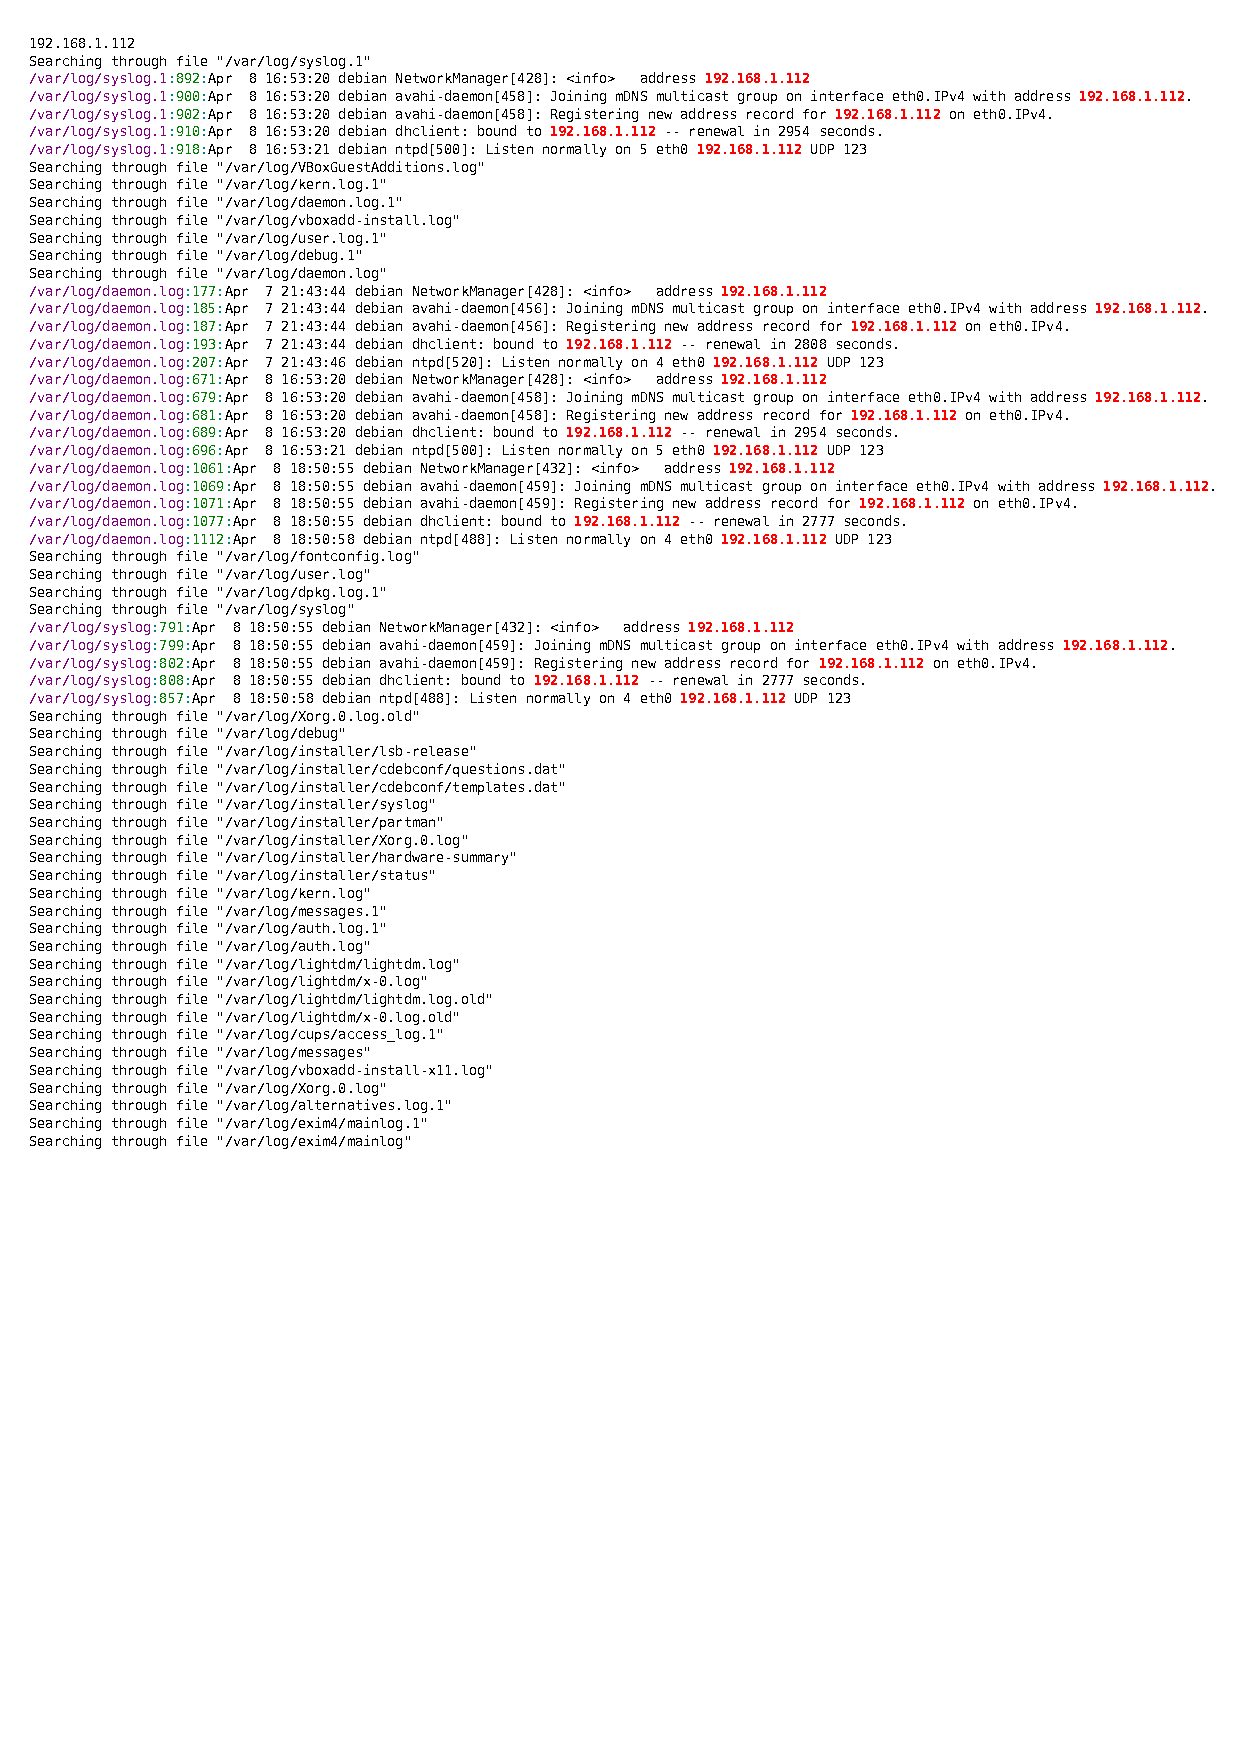
\includegraphics[scale=0.85]{include/sh_1-grep-logs-sh_output.pdf}
  \caption{Körning av programmet i Programlistning~\ref{listing:sh_1-grep-logs.sh}.}
  \label{fig:sh_1-grep-logs.sh_output}
\end{figure}

Bland resultaten finns omnämnanden av \texttt{mDNS} som rör \texttt{DHCP}.
Instruktionerna nämner också att den grafiska miljön har verktyg för att
konfigurera nätverksinställningar, en skärmdump på detta visas i
Figur~\ref{fig:scr_1-network_A} och Figur~\ref{fig:scr_1-network_B} .

\begin{figure}[htp]
  \centering 
  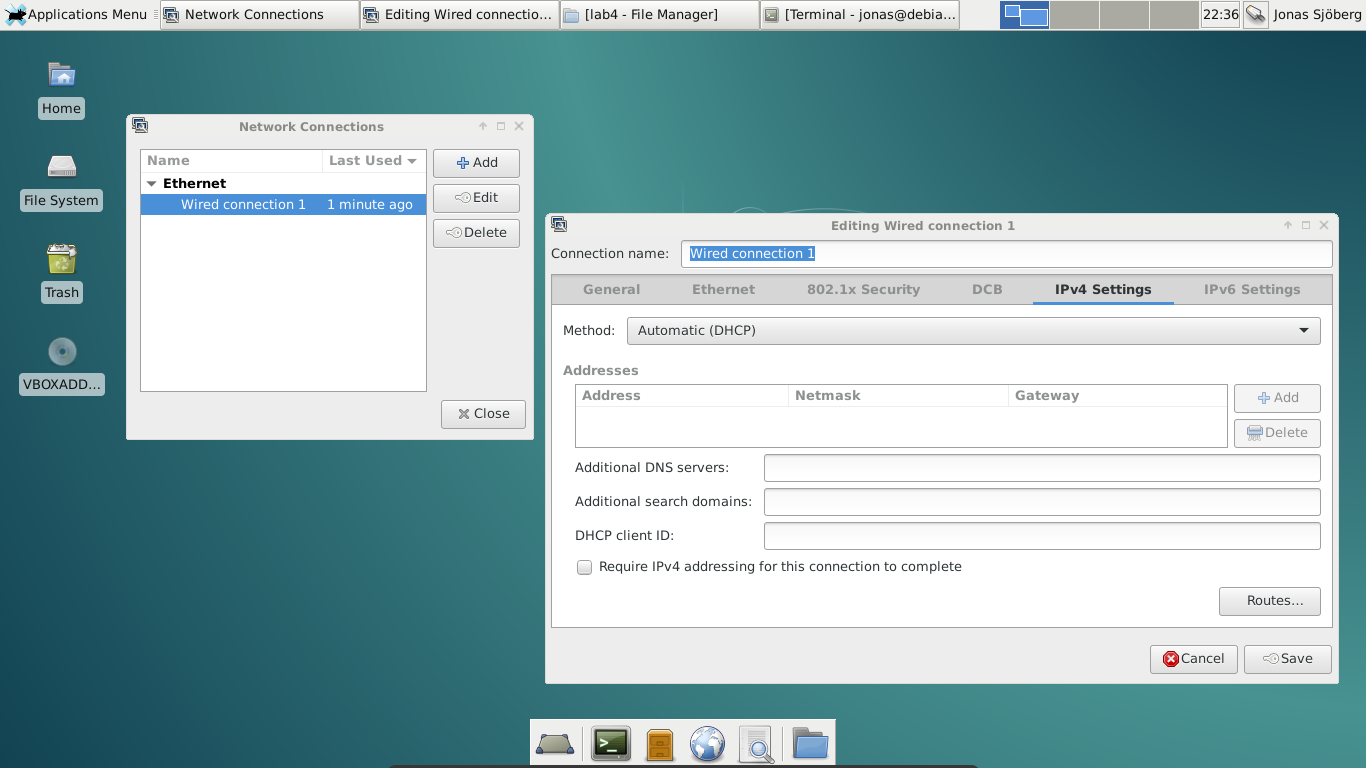
\includegraphics[scale=0.35]{include/scr_1-network_A.png}
  \caption{Nätverksinställningar i det grafiska gränssnittet.}
  \label{fig:scr_1-network_A}
\end{figure}

\begin{figure}[htp]
  \centering 
  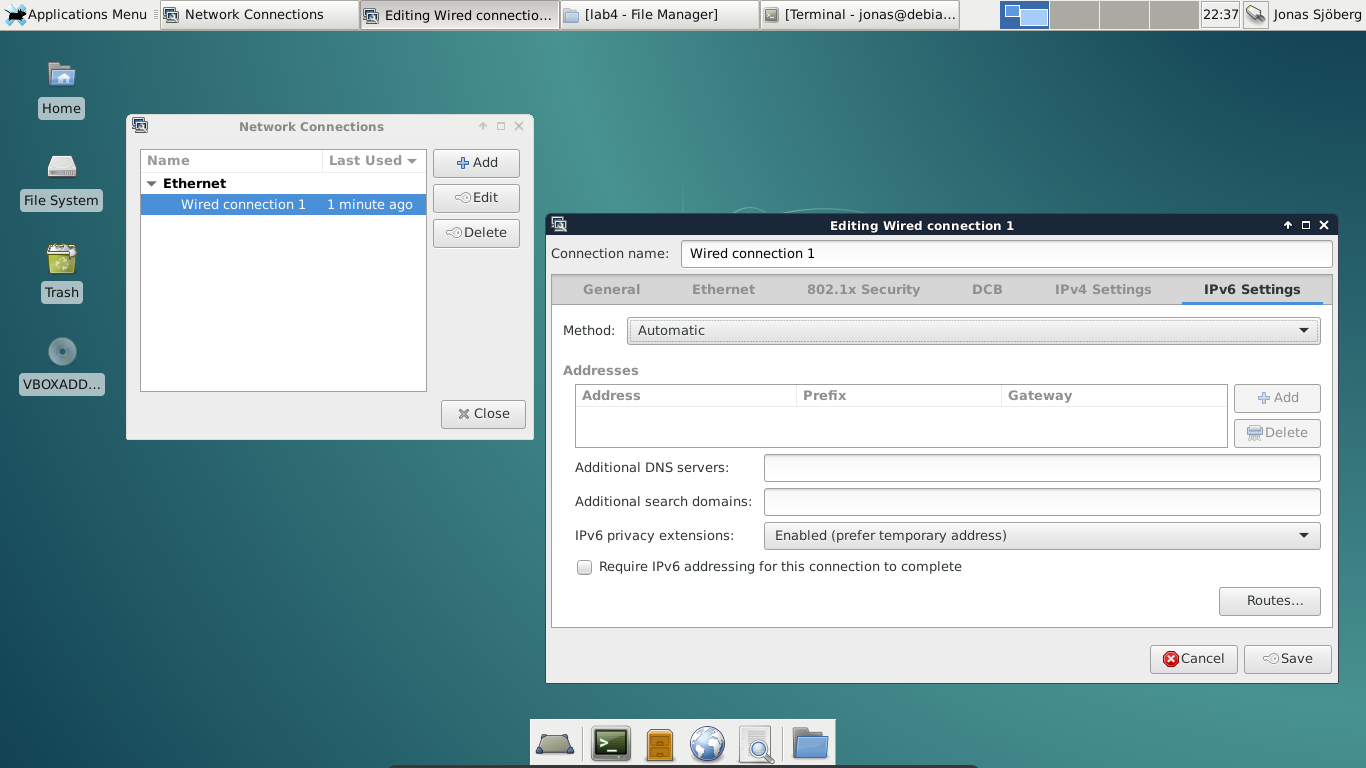
\includegraphics[scale=0.35]{include/scr_1-network_B.png}
  \caption{Nätverksinställningar i det grafiska gränssnittet.}
  \label{fig:scr_1-network_B}
\end{figure}


% ______________________________________________________________________________
\subsection{Nät- och Nodnummer}
\subsubsection{Uppgiftsbeskrivning}
Uppgiften är här att ange vilken nätadress man har genom att använda
\texttt{CIDR} och dessutom ange nätmasken.


\subsubsection{Lösning}
% TODO: Beskriv lösningen av uppgiften ..


% ______________________________________________________________________________
\subsection{Routeradresser}
\subsubsection{Uppgiftsbeskrivning}
Uppgiften är att lista de routrar som maskinen känner till och dessutom ange
vilken som är standardroutern.

\subsubsection{Lösning}
% TODO: Beskriv lösningen av uppgiften ..


% ______________________________________________________________________________
\subsectionM{\texttt{MAC}-adresser}
\subsubsection{Uppgiftsbeskrivning}
Här är uppgiften att lista \texttt{MAC}- och \texttt{IP}-adresser för alla 
maskiner i nätverket.

\subsubsection{Lösning}
% TODO: Beskriv lösningen av uppgiften ..


